\chapter{Results and Discussion}
\label{ch:results_and_discussion}



\section{Statistical Evaluation Methodology}
\label{sec:statistical_evaluation_methodology}

\subsection{The Dem\v{s}ar Statistical Framework}
\label{subsec:demsar_framework}

Comparing several forecasting models across a diverse retail portfolio requires
statistical methods that make no distributional assumptions, so that any apparent
advantage of the graph-augmented architectures reflects a genuine improvement in
forecasting performance rather than random variations. To this end, the framework
of Dem\v{s}ar (2006)~\cite{1248547.1248548} for comparing multiple models over
many datasets was adopted, treating each product as a dataset.

The evaluation is stratified by forecasting head rather than pooling all eight
models into a single ranking. Two pools are tested independently: an LSTM pool
(\texttt{lstm\_baseline}, \texttt{graph2vec\_lstm}, \texttt{gcn\_lstm},
\texttt{gat\_lstm}) and an MLP pool (\texttt{mlp\_baseline},
\texttt{graph2vec\_mlp}, \texttt{gcn\_mlp}, \texttt{gat\_mlp}). Within each pool a temporal baseline is compared against its three graph-augmented variants
(Graph2Vec, GCN, and GAT). This isolates the contribution of the graph signal within
a fixed temporal backbone, and avoids confounding it with differences in the
intrinsic sequence-modelling ability of LSTMs compared to that of MLPs.

A two-stage procedure was applied to each pool. The first stage uses the Friedman
omnibus test to assess whether any statistically significant difference exists
among the models in this pool. If the omnibus test rejects the null hypothesis,
the second stage applies the post-hoc Nemenyi test to identify which pairs of
models account for this difference.

\subsubsection{Friedman Omnibus Test}\label{subsubsec:friedman_test}
The Friedman test is a non-parametric analog of repeated-measures ANOVA. It
is preferred over parametric alternatives because the per-product error
distributions are heterogeneous and non-normal across the catalogue, violating
the assumptions of ANOVA; operating on ranks rather than raw values also makes
the test invariant to large-scale differences between products.

Each statistical block corresponds to a single \emph{(product, seed)} pair: for
every product and seed, the models within a pool are ranked against one another
on the chosen metric (rank one being the lowest error), and each model's average
rank is taken over all blocks, with ties resolved by the mean of the tied ranks.
Crucially, no per-seed or per-product selection is performed --- every seed of
every product contributes, so the comparison reflects the full distribution of
runs rather than a best-case subset, avoiding any optimistic bias from reporting
only the strongest seed of each model.

One caveat is that these blocks are not strictly independent: the
$N_{\text{seeds}}$ runs of a product share the same underlying demand series, so
treating each \emph{(product, seed)} pair as an independent block inflates the
effective sample size (here $60 \times N_{\text{seeds}} = 600$ blocks rather than
$60$) and narrows the Nemenyi critical difference. The reported significance
levels should, therefore, be read as slightly liberal bounds. To assess
sensitivity, the analysis was repeated with each model collapsed to its mean
metric per product, yielding $60$ fully independent blocks
(Table~\ref{tab:perproduct_robustness}). The principal conclusions were
preserved: in both pools the localized GCN and GAT hybrids retained a
statistically significant directional-accuracy (POCID) advantage over the
baseline, and the baselines --- together with the macro-level Graph2Vec
embedding, which retained a significant MAE advantage over the localized hybrids.
The only differences were a small number of marginal pairwise distinctions that
no longer reached significance at the reduced block count: most notably the
macro-level \texttt{graph2vec\_lstm} no longer significantly outperformed the
LSTM baseline on POCID, and two \texttt{graph2vec}-versus-GCN MAE differences
weakened to the $p \approx 0.05$ threshold. These outcomes are consistent with the
wider critical difference at $N=60$ and confirm that the dominant effects are not
an artifact of the product\,$\times$\,seed blocking.

The test evaluates the null hypothesis $H_{0}$ that no difference in average rank
exists among the models in a pool. Unlike repeated-measures ANOVA, it
does not require normality or homogeneity of variance. With $\alpha = 0.05$,
$H_{0}$ is rejected when the Friedman $\chi^{2}$ statistic yields $p < \alpha$,
The post-hoc Nemenyi test was then used to localize the differing pairs.

\begin{table}[ht]
\centering
\caption{Robustness check: average ranks under per-product blocking ($N=60$ independent blocks, each model was averaged over the seeds). Lower is better; the best rank per row is in bold. In every pool the ordering matches the
product\,$\times$\,seed analysis described in Section~\ref{subsec:demsar_framework}. The
only loss of significance relative to that analysis is
\texttt{graph2vec\_lstm} vs.\ \texttt{lstm\_baseline} on POCID.}
\label{tab:perproduct_robustness}
\begin{tabular}{llcccc}
\toprule
Pool & Metric & Baseline & Graph2Vec & GCN & GAT \\
\midrule
LSTM & MAE   & \textbf{1.983} & 2.117 & 2.717 & 3.183 \\
LSTM & POCID & 3.125 & 2.842 & 2.292 & \textbf{1.742} \\
MLP  & MAE   & \textbf{2.050} & 2.183 & 2.783 & 2.983 \\
MLP  & POCID & 2.942 & 2.533 & 2.325 & \textbf{2.200} \\
\bottomrule
\end{tabular}
\end{table}

\subsubsection{Post-hoc Nemenyi Analysis}
\label{subsubsec:posthoc_nemenyi}

If the Friedman test successfully rejects the null hypothesis, the analysis proceeds to the second step: the post hoc Nemenyi test. This test was designed to identify specific architectural pairings that exhibited significant performance differences while strictly controlling the family wise error rate associated with multiple comparisons.

The Nemenyi test calculates a Critical Difference (CD) threshold based on the number of models being compared and the total number of datasets (items). The performance of any two models is considered statistically significantly different if, and only if, the absolute difference between their average ranks is equal to or strictly greater than the CD threshold. This highly conservative approach provides statistically rigorous evidence of whether the proposed graph hybrid genuinely outperforms the standard temporal baseline.
\subsection{Spearman Results and Discussion}
\label{subsec:spearman_results}

In this section, we detail the results of our tests that used the Spearman rank-correlation coefficient to determine the similarity of time series. We will also compare how well each model captures the temporal behavior of the entire portfolio of stores based on their base architecture.

\subsubsection{LSTM Architectures}
\label{subsubsec:spearman_lstm}

The evaluation of the LSTM-based architectures examines whether injecting structural demand relationships, derived from the Spearman-thresholded similarity graph, benefits the recurrent temporal forecasting under the MAE criterion. The Friedman omnibus test yielded a test statistic of $114.05$ ($p = 1.47 \times 10^{-24}$), decisively rejecting the null hypothesis of equal performance and confirming significant differences within the LSTM pool.

Contrary to the expectation that spatial context aids forecasting, the post-hoc Nemenyi analysis revealed that the \texttt{lstm\_baseline} and the macro-level \texttt{graph2vec\_lstm} were the top-performing architectures. The \texttt{lstm\_baseline} attained the lowest average rank of $2.180$, but it was not statistically significantly better than \texttt{graph2vec\_lstm} (rank $2.265$, $p = 0.6645$). Both of these models significantly outperformed the localized routing hybrids: \texttt{gcn\_lstm} (rank $2.727$, $p < 0.0001$) and \texttt{gat\_lstm} (rank $2.828$, $p < 0.0001$). This indicates that, under this graph construction, the recurrent encoder captures the relevant temporal dynamics. Although a global macro-embedding does not harm performance, introducing localized node-level spatial signals acts as noise rather than a useful context. Attention-weighted aggregation is the most detrimental: \texttt{gat\_lstm} is the worst ranked model overall. However, as visualized by the connecting horizontal bar in the Critical Difference diagram (Figure ~\ref{fig:cd_diagram_mae_spearman_lstm}), there is no statistically significant difference between gcn\_lstm and gat\_lstm ($\alpha$ = 0.05). This suggests that the learned spatial attention amplifies rather than filters the error introduced by the demand graph. These MAE hierarchies are visualized in the Critical Difference diagram in Figure~\ref{fig:cd_diagram_mae_spearman_lstm}.



Conversely, while structural embeddings offer no advantage in absolute magnitude forecasting, analyzing the directional accuracy (POCID) reveals a starkly contrasting dynamic. The Friedman omnibus test for POCID yielded a highly significant test statistic of $135.45$ ($p = 3.62 \times 10^{-29}$), confirming profound differences in the trend prediction capabilities among the LSTM variants.

The subsequent post-hoc Nemenyi analysis indicated a reversal of the MAE-based ordering when the models were evaluated for directional accuracy (POCID). The \texttt{lstm\_baseline} obtained the highest (worst) average rank of $2.908$. In contrast, the graph-augmented variants consistently achieved lower rankings. The \texttt{gat\_lstm} model achieved the best average rank ($2.112$), followed by \texttt{gcn\_lstm} ($2.343$). The \texttt{graph2vec\_lstm} hybrid ranked third ($2.637$) and significantly outperformed the baseline (\(p = 0.0015\)). Overall, these results suggest that incorporating the topological context improves directional prediction relative to a standalone LSTM. The accompanying figure shows the CD diagram for POCID. Notably, the complete absence of horizontal connecting bars between any of the models demonstrates that all pairwise differences in their ranks are statistically significant ($\alpha = 0.05$). This establishes a strict, unambiguous performance hierarchy where each model is definitively proven to be better or worse than the others in its category.The CD diagram for POCID is shown in Figure~\ref{fig:cd_diagram_pocid_spearman_lstm}.

\begin{figure}[htbp]
    \centering
     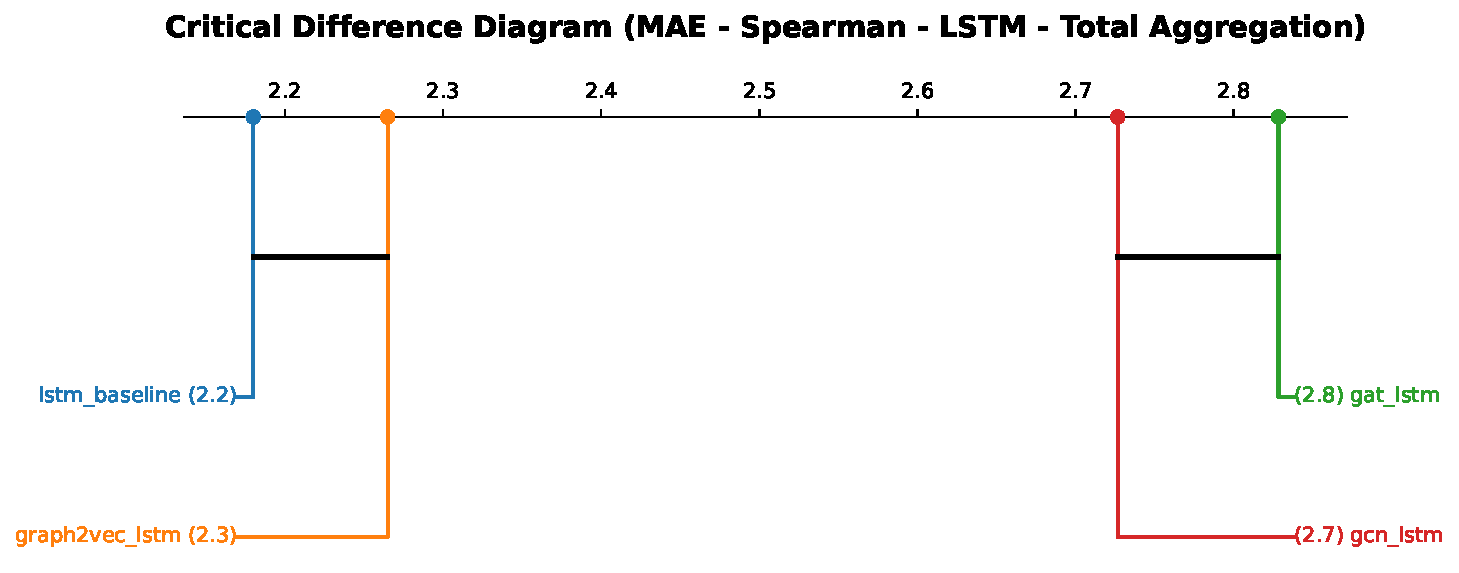
\includegraphics[width=\linewidth]{figures/cd_diagram_mae_spearman_lstm_total.pdf}
    \caption{Critical Difference (CD) diagram for the LSTM-based architectures evaluated on absolute error (MAE) using the Spearman graph. Models connected by a horizontal bar do not possess statistically significant differences ($\alpha = 0.05$).}
    \label{fig:cd_diagram_mae_spearman_lstm}
\end{figure}


\begin{figure}[htbp]
    \centering
     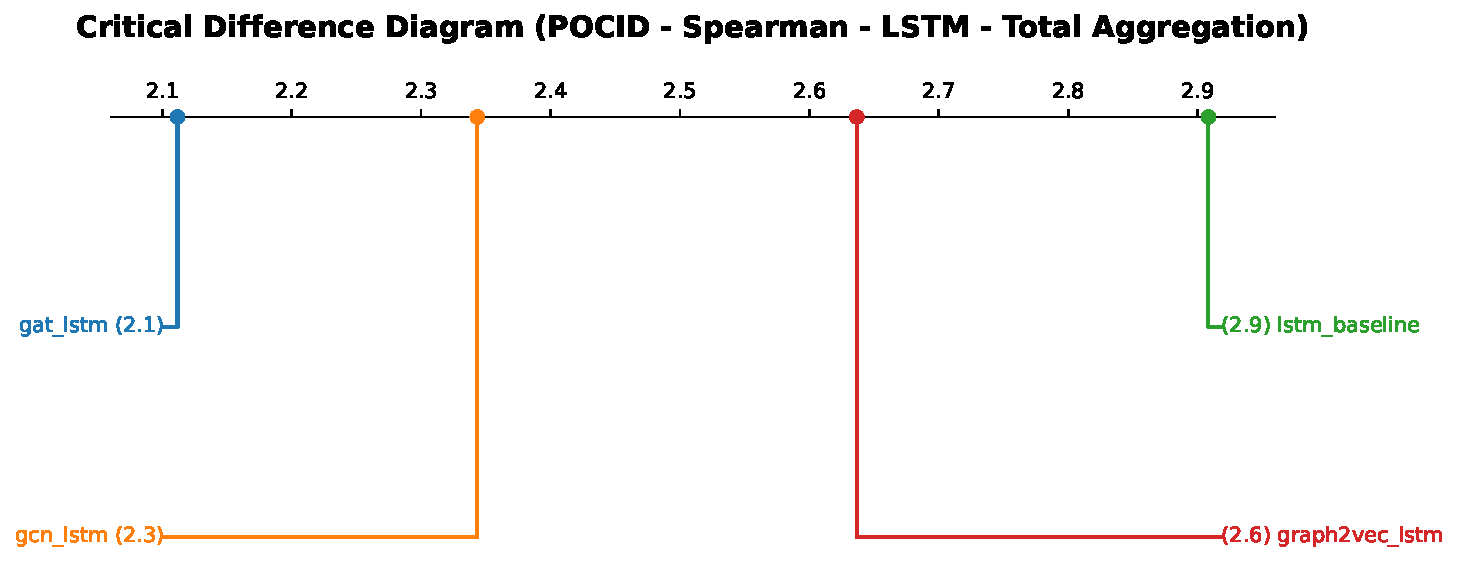
\includegraphics[width=\linewidth]{figures/cd_diagram_pocid_spearman_lstm_total.pdf}
    \caption{Critical Difference (CD) diagram for the LSTM-based architectures evaluated on directional accuracy (POCID) using the Spearman graph. Higher POCID yields lower ranks.}
    \label{fig:cd_diagram_pocid_spearman_lstm}
\end{figure}

Beyond the rank-based Nemenyi analysis, evaluating the mean percentage change in the absolute error (MAE) relative to the \texttt{lstm\_baseline} further quantifies the impact of the structural embeddings. Consistent with the statistical rankings, the integration of the spatial context resulted in a consistent degradation of the magnitude-forecasting accuracy. The macro-level \texttt{graph2vec\_lstm} experienced a minor performance decrease of -1.97\%. However, the localized routing methods suffered more substantial penalties, with the \texttt{gcn\_lstm} and \texttt{gat\_lstm} degrading by -2.88\% and -4.99\%, respectively. This quantifiably confirms that for absolute error, node-level spatial aggregation acts as disruptive noise rather than a constructive context.

In stark contrast, the mean percentage improvements in directional accuracy (POCID) highlight the distinct advantage of the graph-augmented LSTM models. When the objective was shifted to predicting the correct direction of demand movement, the structural hybrids demonstrated clear, quantifiable gains over the baseline. The \texttt{graph2vec\_lstm} achieved a solid +3.66\% improvement. The localized methods leveraged the topological context even more effectively, yielding substantial enhancements: the \texttt{gcn\_lstm} improved by +6.70\%, while the top-ranked \texttt{gat\_lstm} delivered a remarkable +7.93\% increase in trend-prediction accuracy, underlining the power of attention-weighted spatial routing for market inflections.

\subsubsection{MLP Architectures}
\label{subsubsec:spearman_mlp}

A parallel evaluation was conducted for the MLP-based models to assess the impact of graph embeddings on feedforward temporal architectures. First, we evaluated the forecasting performance of the models using the absolute error criterion (MAE). The Friedman omnibus test confirmed global significance within the MLP pool, yielding a test statistic of $117.84$ ($p = 2.25 \times 10^{-25}$).

Mirroring the dynamics observed in the LSTM evaluation, the addition of structural demand relationships did not improve the magnitude forecasting capabilities of the purely feed-forward architectures. The Nemenyi pairwise comparisons indicate that the \texttt{mlp\_baseline} achieved the lowest (best) average rank of $2.178$. However, it is statistically tied to the macro-level \texttt{graph2vec\_mlp} (rank $2.253$, $p = 0.7458$). Both models significantly outperformed the localized spatial routing methods, that is, \texttt{gcn\_mlp} (rank $2.757$, $p < 0.0001$) and \texttt{gat\_mlp} (rank $2.812$, $p < 0.0001$), which are also statistically tied to each other, indicating that neither localized routing strategy provides a definitive performance advantage over the other in this context. This suggests that the learned spatial attention amplifies, rather than filters, the error introduced by the demand graph. The overarching trend persists: to minimize absolute deviation, raw univariate temporal signals are sufficient, and the Spearman-derived node-level spatial context primarily acts as disruptive noise. These performance hierarchies and statistical ties are visually confirmed by the connecting horizontal bars in the Critical Difference diagram in Figure Figure~\ref{fig:cd_diagram_mae_spearman_mlp}.

However, when evaluating the models based on directional accuracy (POCID), the structural embeddings once again demonstrate their value. The Friedman test for POCID across the MLP pool resulted in a highly significant rejection of the null hypothesis (Test Statistic = $38.73$, $p = 1.98 \times 10^{-8}$).

The subsequent post-hoc Nemenyi analysis revealed a reversal of the absolute error hierarchy. Localized graph-augmented architectures excel in predicting demand trends rather than precise volumes. The \texttt{gat\_mlp} hybrid secured the top rank ($2.343$), closely followed by the \texttt{gcn\_mlp} ($2.357$). Conversely, the standalone \texttt{mlp\_baseline} falls to the worst average rank of $2.731$, being significantly outperformed by the \texttt{gcn\_mlp} architecture ($p < 0.0001$) and its attention-weighted counterpart. The macro-level \texttt{graph2vec\_mlp} embedding bridges the gap between the localized methods and the baseline, achieving a rank of $2.568$.

This consistency across both recurrent (LSTM) and feed-forward (MLP) base architectures provides compelling evidence for the core hypothesis of this study: dynamic graph thresholding captures vital structural market movements and trend inflections that standard univariate models remain blind to. The statistical tier list for directional accuracy is confirmed by the Critical Difference diagram in Figure~\ref{fig:cd_diagram_pocid_spearman_mlp}.

\begin{figure}[htbp]
    \centering
    
\includegraphics[width=\linewidth]{figures/cd_diagram_mae_spearman_mlp_total.pdf}
    \caption{Critical Difference (CD) diagram for the MLP-based architectures evaluated on absolute error (MAE) using the Spearman graph. Models connected by a horizontal bar do not possess statistically significant differences ($\alpha = 0.05$).}
    \label{fig:cd_diagram_mae_spearman_mlp}
\end{figure}

\begin{figure}[htbp]
    \centering
    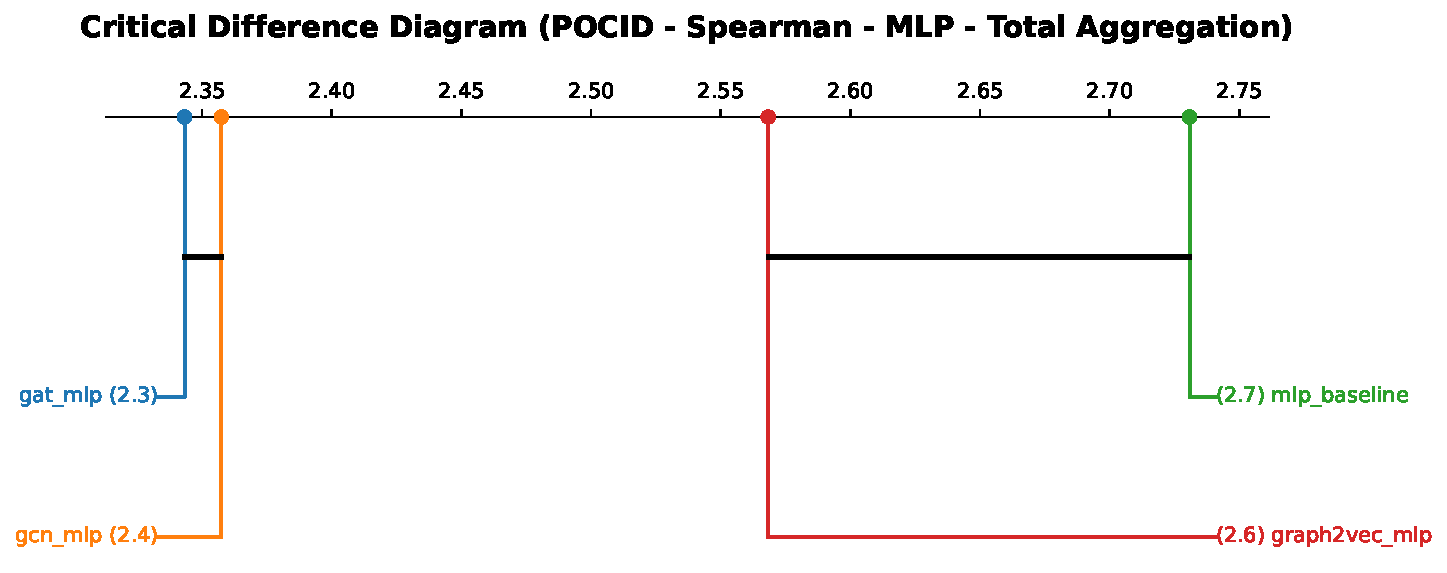
\includegraphics[width=\linewidth]{figures/cd_diagram_pocid_spearman_mlp_total.pdf}
    \caption{Critical Difference (CD) diagram for the MLP-based architectures evaluated on directional accuracy (POCID) using the Spearman graph. Higher POCID yields lower ranks.}
    \label{fig:cd_diagram_pocid_spearman_mlp}
\end{figure}


\newpage


A parallel dynamic is observed within the feedforward architectures when evaluating the absolute error. The mean percentage change in MAE relative to the \texttt{mlp\_baseline} demonstrates quantifiable performance degradation across all structural hybrids. The \texttt{graph2vec\_mlp} saw a modest error increase, degrading by -1.83\%. The localized convolutional and attention variants were penalized more heavily, with the \texttt{gat\_mlp} and \texttt{gcn\_mlp} experiencing performance drops of -3.37\% and -3.76\%, respectively. This perfectly mirrors the LSTM dynamics, proving that raw univariate signals are superior for minimizing the absolute deviation in purely feed-forward setups.

Finally, examining the mean percentage improvements in MLP directional accuracy (POCID) solidifies the value of spatial routing for trend forecasting. Every graph-augmented variant demonstrated clear gains over the standalone \texttt{mlp\_baseline}. The macro-level \texttt{graph2vec\_mlp} yielded a +1.88\% improvement. More impressively, the localized methods drove significant enhancements in predicting demand direction, with the \texttt{gat\_mlp} improving by +3.80\%, and the \texttt{gcn\_mlp} achieving the highest boost at +5.21\%. These percentages reinforce the finding that dynamic graph thresholding is highly effective in capturing synchronized market movements that standard univariate MLPs miss.

\subsection{CID Results and Discussion}
\label{subsec:cid_results}

This section details the statistical evaluation of the models when constructed using the Complexity-Invariant Distance (CID) graph threshold. CID extends the classical Euclidean distance by correcting the intrinsic complexity of each time series and penalizing spurious similarity attributions between structurally dissimilar series. The evaluation follows the same Dem\v{s}ar framework applied to the Spearman graphs, enabling a direct comparison of how the choice of graph construction method affects the model rankings and the statistical conclusions drawn from them.

\subsubsection{LSTM Architectures}
\label{subsubsec:cid_lstm}

Under the CID graph, the evaluation of LSTM-based architectures for magnitude forecasting (MAE) yielded a decisively significant Friedman omnibus test: statistic of $60.56$ ($p = 4.47 \times 10^{-13}$), strongly rejecting the null hypothesis.

The resulting Nemenyi analysis mirrors the Spearman hierarchy but considerably sharpens the tier separation. The \texttt{lstm\_baseline} again leads with the lowest average rank of $2.258$, statistically tied with \texttt{graph2vec\_lstm} (rank $2.352$, $p = 0.5935$). Crucially, both of these top-tier models now significantly outperform \textit{both} localized routing methods at a higher confidence level than Spearman: \texttt{gcn\_lstm} (rank $2.618$, $p < 0.001$) and \texttt{gat\_lstm} (rank $2.772$, $p < 0.0001$). The CID graph thus amplifies the penalty incurred by node-level spatial aggregation; the more structurally discriminating similarity measure introduces graph edges that carry greater noise for the recurrent magnitude estimator. The CD diagram for the MAE is shown in Figure~\ref{fig:cd_diagram_mae_cid_lstm}.


Directional accuracy (POCID) analysis under the CID graph delivered the strongest statistical signal for any configuration tested. The Friedman omnibus test yields a test statistic of $120.52$ ($p = 5.95 \times 10^{-26}$), and the post-hoc Nemenyi analysis reveals a markedly cleaner two-tier structure than was observed under Spearman. The localized graph-augmented architectures form a clearly dominant tier: \texttt{gat\_lstm} leads with an average rank of $2.113$, and \texttt{gcn\_lstm} follows at $2.346$ --- these two are themselves significantly different ($p = 0.0098$), indicating that attention-weighted spatial routing is superior to convolutional routing for trend prediction under this graph. Both architectures significantly outperformed all other models at $p < 0.0001$.

The bottom tier consists of \texttt{graph2vec\_lstm} (rank $2.732$) and \texttt{lstm\_baseline} (rank $2.808$), which are statistically indistinguishable from each other ($p = 0.7392$). This marks a notable departure from the Spearman results, where \texttt{graph2vec\_lstm} achieved a statistically significant edge over the baseline ($p = 0.0161$). Under CID, the macro-level global embedding loses this marginal advantage, suggesting that the more granular similarity measure in CID diminishes the usefulness of the coarse graph2vec representation while simultaneously strengthening the signal extracted by the localized GCN and GAT routing. The CD diagram for the POCID is shown in Figure~\ref{fig:cd_diagram_pocid_cid_lstm}.

\begin{figure}[htbp]
    \centering
    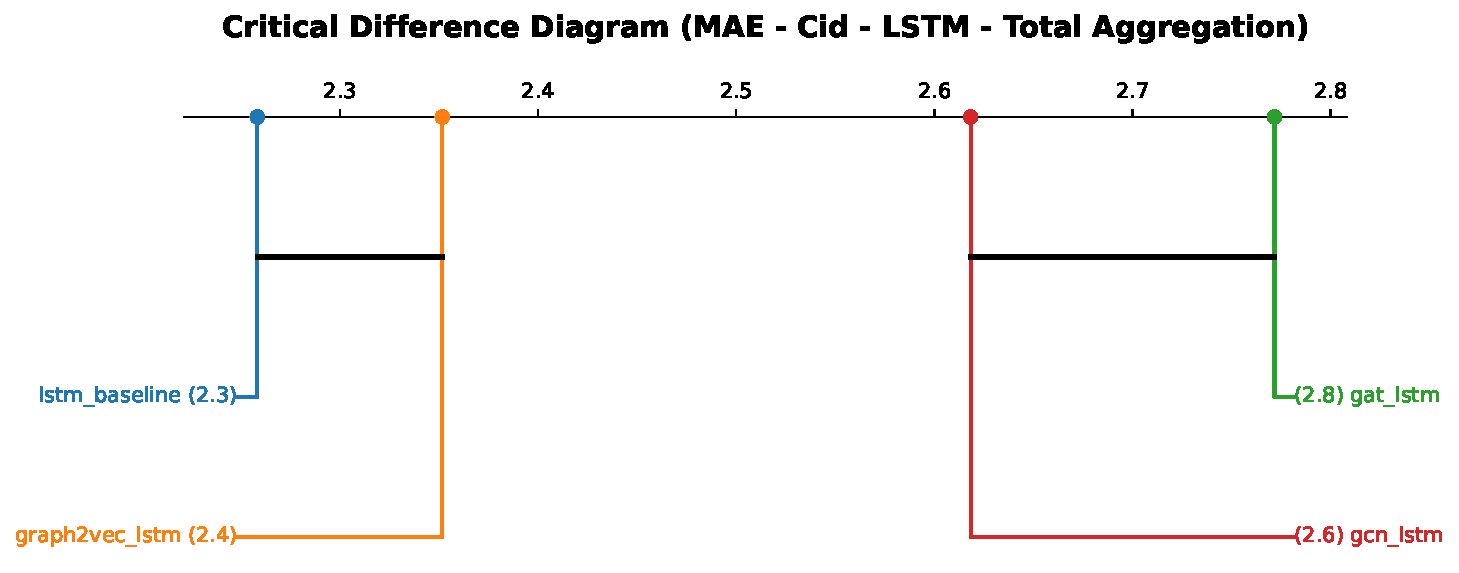
\includegraphics[width=\linewidth]{figures/cd_diagram_mae_cid_lstm_total.pdf}
    \caption{Critical Difference (CD) diagram for the LSTM-based architectures evaluated on absolute error (MAE) using the CID graph. Models connected by a horizontal bar do not possess statistically significant differences ($\alpha = 0.05$).}
    \label{fig:cd_diagram_mae_cid_lstm}
\end{figure}


\begin{figure}[htbp]
    \centering
    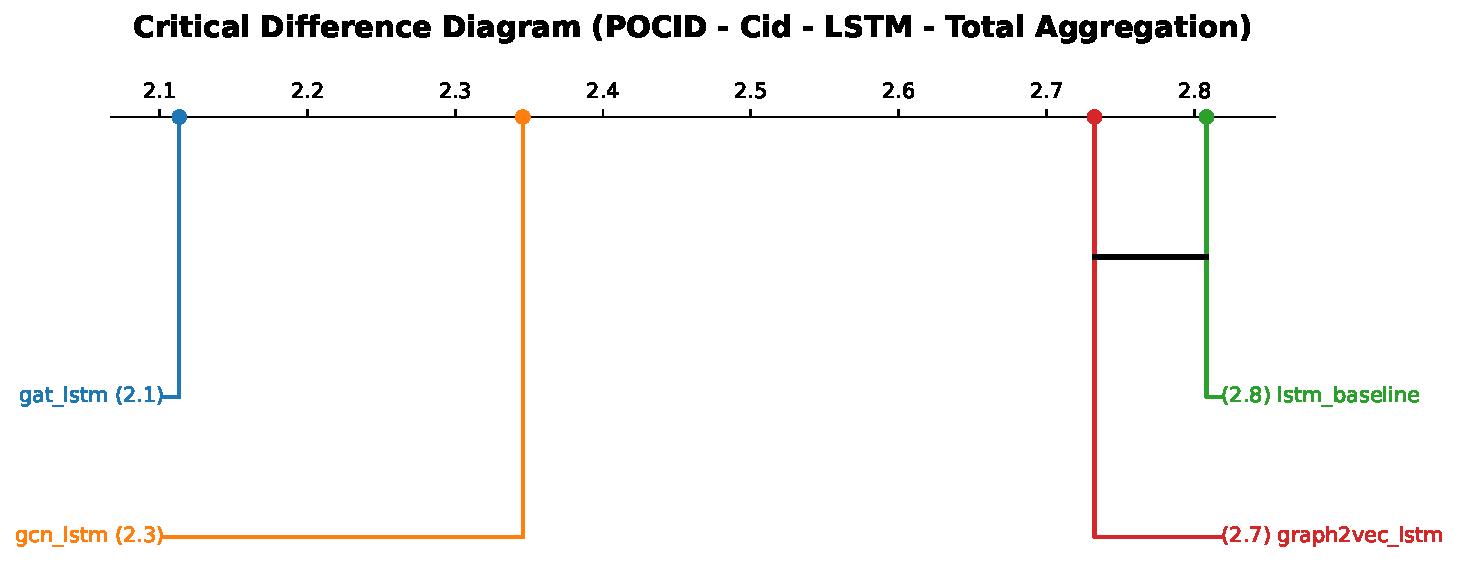
\includegraphics[width=\linewidth]{figures/cd_diagram_pocid_cid_lstm_total.pdf}
    \caption{Critical Difference (CD) diagram for the LSTM-based architectures evaluated on directional accuracy (POCID) using the CID graph. Higher POCID yields lower ranks.}
    \label{fig:cd_diagram_pocid_cid_lstm}
\end{figure}

\newpage
\subsubsection{MLP Architectures}
\label{subsubsec:cid_mlp}

The evaluation of MLP-based architectures under the CID graph reinforces the patterns observed in the LSTM model. For the absolute error (MAE), the Friedman omnibus test yielded a test statistic of $111.18$ ($p = 6.10 \times 10^{-24}$), confirming highly significant differences within the feed-forward pool.

The Nemenyi post-hoc analysis reproduces Spearman ordering exactly. The \texttt{mlp\_baseline} achieved the best average rank of $2.143$, statistically tied with \texttt{graph2vec\_mlp} (rank $2.317$, $p = 0.0923$). The localized architectures are relegated to the bottom tier: both \texttt{gcn\_mlp} (rank $2.737$) and \texttt{gat\_mlp} (rank $2.803$) are significantly outperformed by the baseline and \texttt{graph2vec\_mlp} ($p < 0.0001$ in all cases). The robustness of this finding across both graph construction methods confirms that to minimize absolute deviation, node-level graph routing introduces consistent noise regardless of whether the graph edges are defined by Spearman or CID similarity. The corresponding CD diagram is presented in Figure~\ref{fig:cd_diagram_mae_cid_mlp}.

\begin{figure}[htbp]
    \centering
    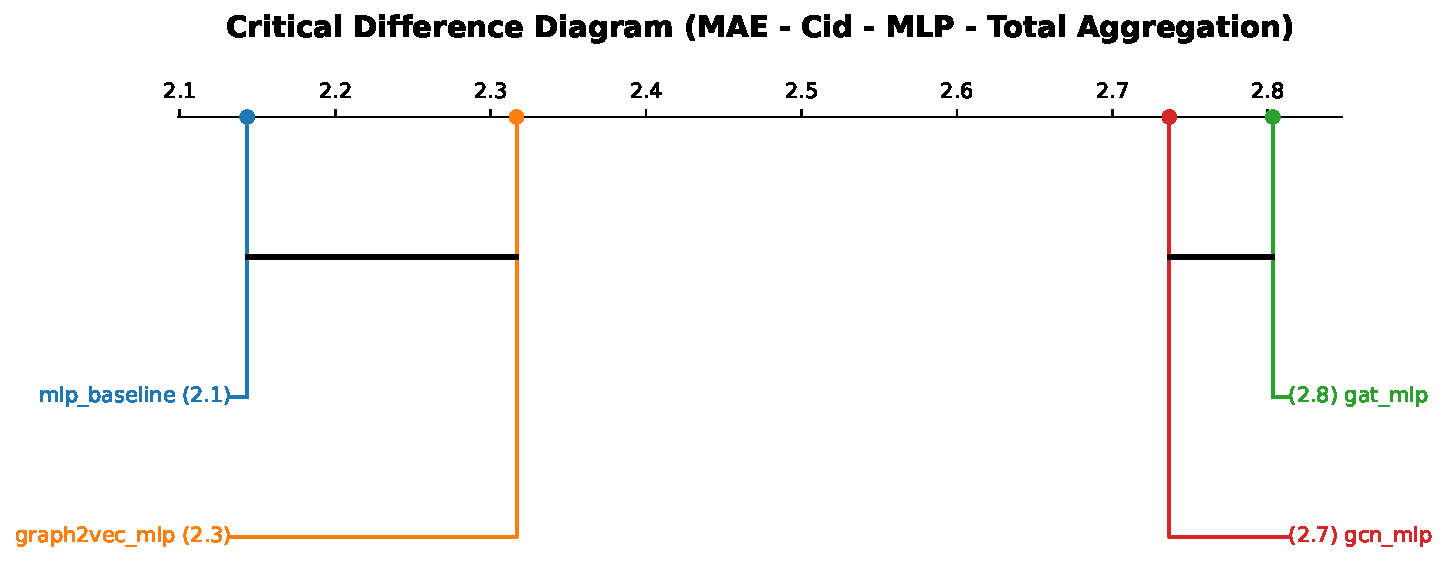
\includegraphics[width=\linewidth]{figures/cd_diagram_mae_cid_mlp_total.pdf}
    \caption{Critical Difference (CD) diagram for the MLP-based architectures evaluated on absolute error (MAE) using the CID graph. Models connected by a horizontal bar do not possess statistically significant differences ($\alpha = 0.05$).}
    \label{fig:cd_diagram_mae_cid_mlp}
\end{figure}

For directional accuracy (POCID), the CID graph produced the weakest omnibus result of the four MLP configurations: a Friedman statistic of $11.20$ ($p = 1.07 \times 10^{-2}$). While the null hypothesis is still rejected, the effect is considerably smaller than that of the Spearman counterpart. The post-hoc Nemenyi analysis revealed that only a single pairwise comparison reached significance: \texttt{gat\_mlp} (rank $2.410$) significantly outperformed the \texttt{mlp\_baseline} (rank $2.641$, $p = 0.0105$). The remaining models, \texttt{graph2vec\_mlp} (rank $2.462$) and \texttt{gcn\_mlp} (rank $2.487$), form a statistically indistinguishable cluster between these two extremes.

This weakened separation under CID for MLP-POCID contrasts with the full four-way ladder observed under Spearman for the same pool and metrics. One plausible interpretation is that the CID-based graph edges, being more sensitive to time-series complexity, encode a stronger and noisier structural prior that homogenizes the intermediate architectures while still providing the attention mechanism of \texttt{gat\_mlp} with a sufficient useful signal to outperform the baseline. The directional accuracy ranking under the CID graph is shown in Figure~\ref{fig:cd_diagram_pocid_cid_mlp}.

\begin{figure}[htbp]
    \centering
    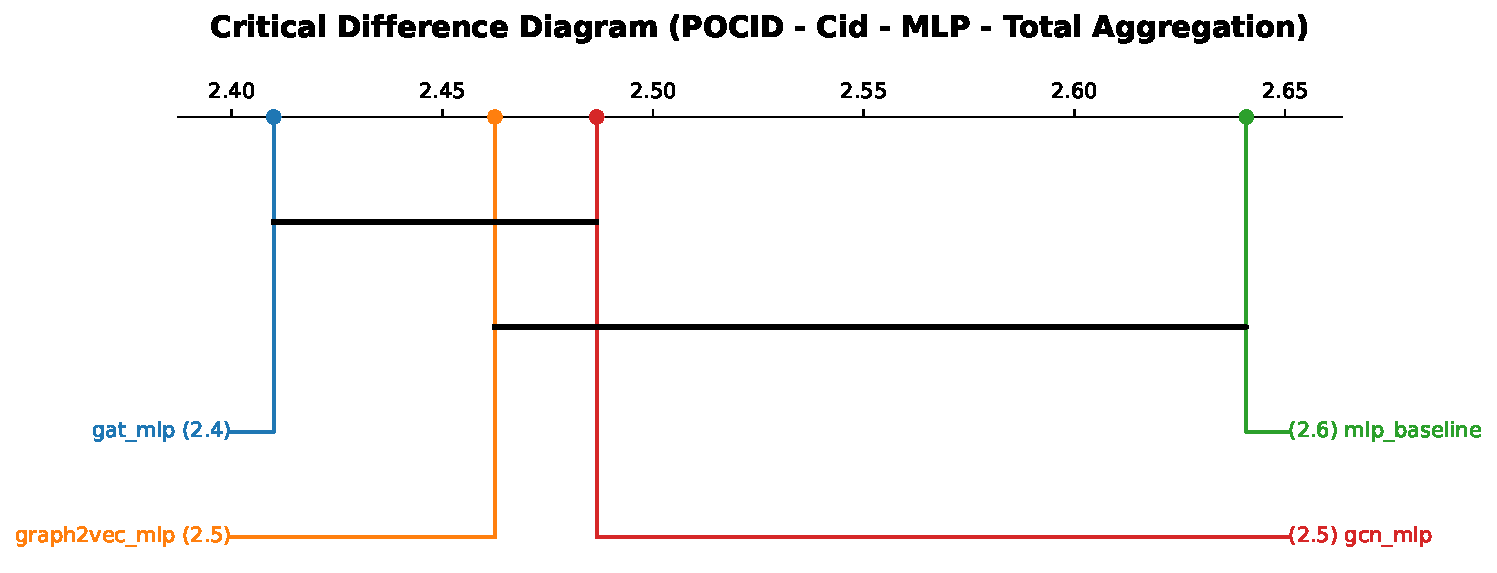
\includegraphics[width=\linewidth]{figures/cd_diagram_pocid_cid_mlp_total.pdf}
    \caption{Critical Difference (CD) diagram for the MLP-based architectures evaluated on directional accuracy (POCID) using the CID graph. Higher POCID yields lower ranks.}
    \label{fig:cd_diagram_pocid_cid_mlp}
\end{figure}

Taken together, the CID results corroborate the major conclusions drawn from the Spearman analysis. In fact, baselines and macro-level graph embeddings lead to MAE, whereas localized GCN and GAT hybrids dominate POCID. The primary effect of switching from Spearman to CID is not a reversal of model rankings but a sharpening of the tier boundaries, most dramatically in the LSTM POCID experiment, where CID produces a cleaner two-tier structure, and a weakening in the MLP POCID experiment, where fewer pairwise differences survive the conservative Nemenyi threshold. This cross-metric consistency across two structurally distinct graph construction methods provides strong evidence that the observed performance dynamics are a property of the model architectures and their interaction with the graph topology, rather than an artifact of a particular similarity measure.

\subsection{Product-level Analysis}
\label{subsec:product_level_analysis}

The heatmaps presented in this section reveal considerable heterogeneity across the
60 products: graph-augmented hybrids offer meaningful gains for a subset of
products, while for others, the baseline is difficult to beat.

Unlike the rank-based Friedman--Nemenyi analysis of
Section~\ref{subsec:demsar_framework}, which aggregates over \emph{every} seed of
every product and is the sole basis for the statistical claims in this chapter, the
product-level view presented here is \emph{descriptive and exploratory}. For each product, every model is summarized by its own best-performing seed, the baseline by the seed that minimized its MAE, and each hybrid likewise by its strongest seed.
This best-seed reduction is applied \emph{symmetrically} to baselines and hybrids,
so the per-product comparison remains like-for-like: a hybrid must beat the baseline
even when both are shown at their best performance. It is, however, a best-case summary rather
than a significance test --- the percentages reported below are computed on the test
horizon and are intended only to characterise \emph{which} products benefit from
relational structure, and by approximately how much. No statistical conclusions are drawn
from them; all significance results in this work derive exclusively from the
all-seeds analysis of Section~\ref{subsec:demsar_framework} and the conservative
per-product robustness check in Table~\ref{tab:perproduct_robustness}. This section
highlights the most consistent winners and losers under this protocol.

\subsubsection*{Best-Performing Products Using Spearman}
\textbf{Product 915640} stands out as the product that benefits most from graph
augmentation for error reduction. Across all three LSTM hybrids the MAE
improvement over the baseline reaches \(+15.5\%\), \(+20.8\%\), and \(+23.4\%\)
respectively (Figures~\ref{fig:heatmap_spearman_lstm_mae_p1}--\ref{fig:heatmap_spearman_lstm_mae_p2}),
and the MLP family echoes the same pattern with gains of \(+13.0\%\), \(+21.5\%\),
and \(+20.5\%\) (Figures~\ref{fig:heatmap_spearman_mlp_mae_p1}--\ref{fig:heatmap_spearman_mlp_mae_p2}).
The graph signal therefore contributes consistently and substantially for this product
regardless of the choice of the forecaster backbone. The directional accuracy (POCID),
however, does not follow the same trend — POCID improvements are modest or slightly
negative for this product (Figures~\ref{fig:heatmap_spearman_lstm_mae_p1}--\ref{fig:heatmap_spearman_lstm_pocid_p2},
\ref{fig:heatmap_spearman_mlp_pocid_p1}--\ref{fig:heatmap_spearman_mlp_pocid_p2}) — suggesting that
the graph embedding helps the model reduce magnitude error without fully correcting
directional bias.

\textbf{Product 921558} shows reliable MAE gains across both families
(\(\approx +8\%\) for LSTM, \(\approx +14\%\) for MLP
Figures~\ref{fig:heatmap_spearman_lstm_mae_p2}, \ref{fig:heatmap_spearman_mlp_mae_p2}) and
simultaneously benefits from strong POCID improvements in the LSTM family
(\(+7.6\%\) to \(+19.0\%\); Figure~\ref{fig:heatmap_spearman_lstm_pocid_p2}), making it
one of the few products where graph augmentation improves both accuracy metrics
together under an LSTM backbone.

\textbf{Product 908786} achieves the largest LSTM MAE gains overall (\(+14.0\%\),
\(+17.2\%\), \(+13.9\%\); Figure~\ref{fig:heatmap_spearman_lstm_mae_p1}), with the
improvement uniformly distributed across all three hybrids, indicating that the
graph structure rather than a specific architecture that drives the benefit.

\textbf{Product 500056} and \textbf{product 933457} are notable from a directional
accuracy standpoint: in the LSTM POCID heatmap
(Figures~\ref{fig:heatmap_spearman_lstm_mae_p1}--\ref{fig:heatmap_spearman_lstm_mae_p1}) both
products show consistently positive improvements across all three hybrids
(\(+17.4\%\), \(+20.7\%\), \(+15.2\%\) and \(+3.2\%\), \(+22.3\%\), \(+22.3\%\)
respectively), suggesting the graph neighbourhood encodes useful directional
co-movement signals for these commodities.

\subsubsection*{Worst-Performing Products}
\textbf{Product 26002} is the clearest case of consistent graph-induced degradation.
In the LSTM MAE heatmap (Figure~\ref{fig:heatmap_spearman_lstm_mae_p1}) it records the
largest negative values in the entire dataset (\(-54.3\%\), \(-28.9\%\),
\(-54.6\%\)), meaning the hybrid models roughly double the absolute error relative
to the LSTM baseline. The MLP family shows the same pattern (\(-19.4\%\),
\(-37.9\%\), \(-46.1\%\); Figure~\ref{fig:heatmap_spearman_mlp_mae_p1}). This suggests the
demand signal for product 26002 carries idiosyncratic dynamics that are poorly
served — and possibly harmed — by the cross-product graph prior injected via the
embedding $z$.

\textbf{Product 26220} is the dominant outlier in the MLP family, with MAE
degradation of \(-28.4\%\), \(-31.2\%\), and \(-25.2\%\) across all three MLP
hybrids (Figure~\ref{fig:heatmap_spearman_mlp_mae_p1}), the most uniformly negative row
in that heatmap.

\textbf{Product 6032} suffers consistently in both MAE heatmaps
(LSTM: \(-36.9\%\), \(-12.0\%\), \(-45.9\%\), Figure~\ref{fig:heatmap_spearman_lstm_mae_p1};
MLP: \(-7.6\%\), \(-15.7\%\), \(-16.5\%\), Figure~\ref{fig:heatmap_spearman_mlp_mae_p1}),
reinforcing the pattern that certain products are structurally incompatible with
the graph augmentation strategy.

Products that benefit from graph augmentation tend to do so uniformly across all
three hybrid architectures (Figures~\ref{fig:heatmap_spearman_lstm_mae_p1}--\ref{fig:heatmap_spearman_mlp_pocid_p2}),
implying that the improvement is driven by the graph structure itself rather than
by a specific model design choice. Conversely, products that are harmed also
suffer across all variants, pointing to a product-level characteristic — such as
low co-movement with its graph neighbours, or a predominantly exogenous demand
driver not captured by the graph — as the root cause of degradation. Overall, the
graph signal is beneficial for a minority of products and neutral or harmful for
the majority, consistent with the aggregate statistics reported in
Section~\ref{subsec:demsar_framework}.

\subsubsection*{Best-Performing Products Using CID}

\textbf{Product 915640} is again the strongest beneficiary of graph augmentation for error reduction under the CID similarity measure. The LSTM family yields MAE improvements of (+16.3\%), (+15.8\%), and (+17.3\%) across all three hybrids (Figure~\ref{fig:heatmap_cid_lstm_mae_p2}), and the MLP family mirrors this with gains of (+12.8\%), (+21.8\%), and (+21.2\%) (Figure~\ref{fig:heatmap_cid_mlp_mae_p2}). The uniformity across all six model variants points squarely to the CID-derived graph structure as the source of the gain, rather than any particular architecture choice. As with the Spearman graph, the directional accuracy for this product does not follow suit; POCID changes are small or slightly negative across both families (Figures~\ref{fig:heatmap_cid_lstm_pocid_p2}, \ref{fig:heatmap_cid_mlp_pocid_p2}), confirming that the embedding reduces the magnitude error without correcting the directional bias.

\textbf{Product 921558} stands out as one of the few products that benefits on both metrics simultaneously under an LSTM backbone. The MAE improves by (+6.2\%), (+7.8\%), and (+7.0\%) across the three LSTM hybrids (Figure~\ref{fig:heatmap_cid_lstm_mae_p2}), while POCID improvements reach (+12.7\%), (+20.3\%), and (+10.1\%) (Figure~\ref{fig:heatmap_cid_lstm_pocid_p2}). The MLP family provides further evidence of consistent error reduction ((+14.5\%), (+14.2\%), (+15.5\%); Figure~\ref{fig:heatmap_cid_mlp_mae_p2}), making this product a reliable beneficiary of CID-based graph augmentation across both backbone types and evaluation metrics.

\textbf{Product 13544} is notable for combining moderate LSTM MAE gains ((-0.4\%), (+13.1\%), (+15.3\%); Figure~\ref{fig:heatmap_cid_lstm_mae_p1}) with the strongest MLP MAE improvements in the first product block ((+21.5\%), (+25.8\%), (+20.8\%); Figure~\ref{fig:heatmap_cid_mlp_mae_p1}). Its LSTM POCID is also consistently positive ((+12.6\%), (+6.3\%), (+15.8\%); Figure~\ref{fig:heatmap_cid_lstm_pocid_p1}), indicating that the CID neighborhood for this product encodes co-movement information that translates into genuine directional improvement for the LSTM-based models.

\textbf{Product 904144} presents the most striking directional accuracy improvements in the entire CID analysis. Its LSTM POCID gains reach (+16.3\%), (+26.5\%), and (+30.6\%) — the highest values observed in the LSTM POCID heatmap (Figure. ~\ref{fig:heatmap_cid_lstm_pocid_p2}). However, the MAE picture is reversed, with the error increasing by (-13.0\%), (-15.1\%), and (-18.1\%) across the same models (Figure~\ref{fig:heatmap_cid_lstm_mae_p2}). This trade-off — sharply improved direction prediction at the cost of larger absolute errors — suggests that the CID graph embedding shifts the model towards a sign-correct but magnitude-inaccurate forecasting regime for this product.

\textbf{Product 933457} is the most reliable directional beneficiary across both backbone families. The LSTM POCID improvements are (+17.0\%), (+21.3\%), and (+26.6\%) (Figure~\ref{fig:heatmap_cid_lstm_pocid_p2}), and the MLP family sustains the pattern with (+12.8\%), (+19.8\%), and (+7.0\%) (Figure~\ref{fig:heatmap_cid_mlp_pocid_p2}). MAE changes are slightly negative but small (within (-2\%) to (-4\%) across models), so the graph signal provides a net directional benefit with a minimal accuracy cost for this product.

\subsubsection*{Worst-Performing Products Using CID}

\textbf{Product 26002} is the most damaging case in the CID analysis, and by a substantial margin. The LSTM MAE heatmap records improvements of (-49.2\%), (-55.6\%), and (-43.5\%) (Figure~\ref{fig:heatmap_cid_lstm_mae_p1}) — the three most extreme negative values in the entire dataset — implying that the hybrid models produce errors approximately 1.5$\times$ that of the LSTM baseline. The MLP family is equally affected: (-21.3\%), (-43.0\%), and (-45.0\%) (Figure~\ref{fig:heatmap_cid_mlp_mae_p1}). The degradation is total and architecture-agnostic, pointing to a product with demand dynamics that are so idiosyncratic that the CID-derived cross-product prior is actively harmful, regardless of how the embedding is consumed.

\textbf{Product 26220} is the second most consistently degraded product in the CID experiment. The MAE worsens by (-25.2\%), (-22.8\%), and (-20.7\%) for all three LSTM hybrids (Figure~\ref{fig:heatmap_cid_lstm_mae_p1}) and by (-26.8\%), (-23.3\%), and (-13.8\%) for the MLP family (Figure~\ref{fig:heatmap_cid_mlp_mae_p1}). The uniformity across both forecast heads confirms this as a product-level incompatibility with the graph structure, rather than a model-specific failure.

\textbf{Product 6032} presents a dissociation between the two metrics that is unique among the worst performers. Its LSTM MAE degrades substantially across all three hybrids ((-25.9\%), (-23.6\%), (-30.2\%); Figure~\ref{fig:heatmap_cid_lstm_mae_p1}), yet its LSTM POCID is strongly positive ((+14.4\%), (+22.7\%), (+18.6\%); Figure~\ref{fig:heatmap_cid_lstm_pocid_p1}) — among the largest directional improvements in the dataset. This inversion suggests that the CID graph embedding conveys a directional co-movement signal that is genuinely useful for predicting the sign of change but simultaneously introduces a bias that inflates the absolute forecast error. Therefore, the product is a boundary case in which the graph is informative in a narrow sense but harmful in the aggregate.

As shown in the Spearman graph, the cross-architecture consistency of both gains and losses under CID points to the product's graph neighborhood — its assigned co-movement peers — as the primary determinant of whether augmentation helps or hurts, rather than any property of the model architecture itself.


\section{Scalability Analysis}
\label{sec:scalability}

To assess the practical cost of deploying each model at scale, we ran a scalability
benchmark in which every model variant processes a growing number of products
sequentially, from a single product to $n=500$. For each product we record the
graph construction time (\texttt{build\_s}), the training time (\texttt{train\_s}),
the inference time (\texttt{infer\_s}), and the number of epochs to convergence
(\texttt{epochs\_trained}). Eight variants are compared: two graph-free baselines
(\texttt{lstm\_baseline}, \texttt{mlp\_baseline}) and six graph-based models pairing
each of three neighbourhood encoders (Graph2Vec, GCN, GAT) with an LSTM or an MLP
forecasting head.

\subsection*{CPU-bound behaviour and memory profiling limitations}

All experiments were performed on a CPU. This choice is not merely a hardware constraint; given the pipeline architecture, CPU execution is the natural fit. The rationale comprises three parts: graph construction, data loading, and model capacity.

\paragraph{Graph construction.}
For each product, a neighborhood graph was constructed by computing Spearman correlations between the target series and every other series in the catalogue over a 30-day sliding window. This is a dense $\mathcal{O}(N_{\text{catalogue}} \cdot T)$ operation implemented in NumPy/SciPy, and it is not readily expressed as a GPU-friendly batched tensor kernel in the implementation. Node features are then extracted in \texttt{catch24\_minmaxlast} mode via \texttt{pycatch22}, a native C extension that evaluates 24 time-series statistics per node (one series at a time). For the Graph2Vec variants, the Doc2Vec embedding was trained with Gensim, again on the CPU. These preprocessing stages do not naturally yield large contiguous tensors for GPU streaming and dominate the wall-clock time per product.

\paragraph{Data loading and mini-batch geometry.}
Even during neural training, a bottleneck remains on the host. The per-step collation strategy (\texttt{collate\_pyg\_ts}) assembles $B \times L = 32 \times 30 = 960$ individual \texttt{Data} ego-graphs per mini-batch by calling \texttt{Batch.from\_data\_list()} within the DataLoader worker. Most ego-graphs contain 2--10 nodes under the Spearman threshold of 0.634, yielding very small, irregular sparse adjacencies. Transferring 960 variably shaped micrographs over PCIe per step would introduce transfer and launch overheads that are likely to exceed the useful GPU compute at this scale. In practice, GPU sparse kernels are most effective when operating on larger, more regular batches; a 5-node ego graph provides insufficient arithmetic intensity to amortize overheads.

\paragraph{Model capacity.}
The neural components were intentionally lightweight: a 2-layer GCN or GAT (hidden dimension 32, output dimension 16) paired with either a single-layer LSTM (hidden size 32) or a time-distributed MLP with widths (128, 64). The total parameter count per model was in the low thousands. At this scale, CPU BLAS (e.g., OpenBLAS/MKL) is typically competitive end-to-end once host--device transfer latency is accounted for, because the compute-to-transfer ratio rarely reaches a regime where GPU parallelism dominates.

\paragraph{Memory profiling.}
Together, these factors complicate accurate peak memory measurements. Python-level tools such as \texttt{tracemalloc} or \texttt{memory\_profiler} instrument only the Python allocator and miss PyTorch's caching allocator: freed tensor buffers may be retained in a reuse pool rather than returned to the OS, so the Python-visible heap can understate true consumption. Conversely, the OS-level resident set size (RSS) can overstate it: products are processed sequentially, whereas the OS page cache for the datasets can accumulate across products and is not necessarily released between iterations. In addition, \texttt{pycatch22} and the Gensim Doc2Vec model use off-heap allocations that neither approach captures. Therefore, this study uses wall-clock time, split into \texttt{build\_s}, \texttt{train\_s}, and \texttt{infer\_s}, as the primary scalability metric. A GPU-based deployment at a larger scale (e.g., parallel product processing with batched graph construction) would also make memory tracking more tractable via \texttt{torch.cuda.max\_memory\_allocated()}, but that is outside the scope of the present single-product sequential evaluation.
% ── Cumulative training cost ─────────────────────────────────────────────
\subsection{Cumulative Training Cost}
\label{sec:scalability-train}

Figure~\ref{fig:cum-train} shows the cumulative training time as the workload increases.
All curves are close to linear in $n$, confirming that per-product training cost is
roughly constant and that no variant exhibits super-linear blow-up as the catalogue
grows. The variants were separated into three clear tiers. The graph-free baselines are the
cheapest by a wide margin ($\approx 7{,}000$s for the full $500$ products, that is
$\approx 14$\,s per product). The Graph2Vec and GCN variants form a middle tier
($\approx 22{,}000$--$40{,}000$\,s). The GAT variants are the most expensive, with
\texttt{gat\_mlp} reaching $\approx 82{,}000$\,s and \texttt{gat\_lstm}
$\approx 62{,}000$\,s, which is roughly an order of magnitude above the baselines.
Therefore, the attention mechanism dominates the training budget. The visible ``steps'' in
the curves correspond to individual products that required substantially more epochs
before the early stopping was triggered.

\begin{figure}[ht]
    \centering
    
\includegraphics[width=0.7\linewidth]{cum_train_evolution.pdf}
    \caption{Cumulative training time as a function of the number of products
    processed ($n$) and one line per model variant. The near-linear growth indicates
    constant per-product cost; the GAT variants are roughly an order of magnitude
    more expensive to train than the graph-free baselines.}
    \label{fig:cum-train}
\end{figure}

% ── Graph construction overhead ──────────────────────────────────────────
\subsection{Graph Construction Overhead}
\label{sec:scalability-build}

Graph construction is a one-off per-product cost shared by all graph-based variants and is absent (zero) for the baselines. Across the graph models, the mean build time is modest and comparable ($\approx 3.0$\,s per product), and it is independent of the forecasting head. Therefore, it is not a scalability bottleneck: graph construction accounts for only a small fraction of the end-to-end cost, which is dominated by training (Section~\ref{sec:scalability-train}).

% ── Inference cost ───────────────────────────────────────────────────────
\subsection{Inference Cost}
\label{sec:scalability-infer}

Cumulative inference time (Figure~\ref{fig:cum-infer}) again grows linearly in $n$,
However, the ordering differs markedly from that of training. Here the Graph2Vec variants are the
most expensive at inference time --- \texttt{graph2vec\_lstm} reaches $\approx 660$\,s
and \texttt{graph2vec\_mlp} $\approx 550$s. It is important to note that all
graph-based variants rebuild the ego-graph from scratch at every forecast step (with
the target node set to the model's own rolling predictions and the neighbours
observed); therefore, this rebuild cost is common to all of them. What sets Graph2Vec
apart is that each rebuilt graph must additionally be \emph{re-embedded} by the
trained model: a Weisfeiler--Lehman relabelling followed by a Doc2Vec
\texttt{infer\_vector} pass --- at every step, whereas the GCN and GAT variants require
only a single forward pass over a rebuilt graph. Consequently the GAT and GCN
variants are cheaper at inference ($\approx 100$--$220$\,s) despite being costlier to
train, and the baselines remained negligible ($\approx 33$\,s). This decoupling of
training and inference cost is relevant for deployment: a model that is expensive to
Train once may still be cheap to serve repeatedly, and vice versa.

\begin{figure}[ht]
    \centering
    
\includegraphics[width=0.7\linewidth]{figures/cum_infer_evolution.pdf}
    \caption{Cumulative inference time as a function of the number of products
    processed ($n$) and one line per model variant. All graph-based variants rebuild the
    ego-graph at every forecast step; the Graph2Vec variants are nonetheless the most
    expensive because each rebuilt graph must additionally be re-embedded by the
    trained model (Weisfeiler--Lehman relabelling followed by a Doc2Vec
    \texttt{infer\_vector} pass) at every step, whereas the GCN/GAT variants require
    only a single GNN forward pass.}
    \label{fig:cum-infer}
\end{figure}


% ── Training efficiency: epochs and per-epoch cost ───────────────────────
\subsection{Training Efficiency: Epochs and Per-Epoch Cost}
\label{sec:scalability-epochs}

To separate \emph{how many} optimisation steps each model needs from \emph{how
expensive} each step is, Table~\ref{tab:scalability-timing} reports the mean number of
epochs required to fit one product and the average wall clock time per epoch.
The mean epoch count is broadly similar across variants ($\approx 125$--$197$), so the
large training-cost differences observed in Section~\ref{sec:scalability-train} are
driven primarily by the per-epoch cost, rather than by slower convergence. The
graph-free baselines cost $\approx 0.04$\,s/epoch, the Graph2Vec variants
$\approx 0.28$\,s/epoch (an order of magnitude more), and the GCN/GAT variants more
still. The high standard deviation in epoch counts (e.g. \texttt{graph2vec\_mlp})
reflects the per-product variability of the early stopping. 
\begin{table}[ht]
\centering
\caption{Per-model scalability statistics over $N=500$ products: mean and std of
per-product training time, mean per-product inference time, and cumulative totals.}
\label{tab:scalability-timing}
\begingroup
\small
\setlength{\tabcolsep}{4pt} % tighten column spacing
\resizebox{\textwidth}{!}{%
\begin{tabular}{lrrrrrrr}
\toprule
Model variant & Mean build (s) & Mean train (s) & Std train (s) & Mean infer (s) & Cum.\ train (s) & Cum.\ infer (s) & $N$ \\
\midrule
    \texttt{lstm\_baseline}   & ---  &  8.20 &   2.89 & 0.170 &  4098 &  85 & 500 \\
    \texttt{mlp\_baseline}    & ---  & 12.00 &   6.74 & 0.240 &  6001 & 120 & 500 \\
    \texttt{graph2vec\_lstm}  & 3.04 & 45.16 &  12.84 & 1.272 & 22578 & 636 & 500 \\
    \texttt{graph2vec\_mlp}   & 3.06 & 68.46 &  40.66 & 1.138 & 34229 & 569 & 500 \\
    \texttt{gcn\_lstm}        & 3.00 & 59.91 &  19.05 & 0.487 & 29955 & 244 & 500 \\
    \texttt{gcn\_mlp}         & 3.04 & 89.63 &  66.65 & 0.471 & 44815 & 236 & 500 \\
    \texttt{gat\_lstm}        & 3.16 & 101.83 & 109.03 & 0.671 & 50913 & 336 & 500 \\
    \texttt{gat\_mlp}         & 2.95 & 140.63 & 196.11 & 0.605 & 70313 & 302 & 500 \\
\bottomrule
\end{tabular}%
}
\endgroup
\end{table}


